\section{Equipment}\label{equipment}
The machine used for the measurement was a Keysight PNA N5227A 4-port \gls{NA} with parallel port capture and supports frequencies from 10 MHz to 67 GHz. The NA has a receiver $DR$ of 131 dB. With a four port NA the antennas can be set in a one TX and three RX configuration. This gives antenna diversity of three. Calibration can be done by connecting the cables together and do a simple normalization, the drawback of this being that a \gls{PA} can not be used. The sweep data will be saved to a USB storage device.


The cables used have a loss of 0.5 $\frac{dB}{m}$. Three 10 m cables and one 4 m cable were used for the RX and TX antennas respectively. This gives a total cable loss, $L_c$, of 7 dB.


The RX antenna array is a omnidirectional antenna with a spacing of $0.4 \lambda$ given a $f_c$ of 5 GHz. The TX antenna is a directional antenna with $G_{TX}=12.7$ dBi at 4.5 GHz and $G_{TX}=10.7$ dBi at 5.5 GHz. The full gain chart of the antenna can be found in \appref{ant_adix}. 

\begin{figure}[H]
  \centering
  \begin{minipage}[H]{0.42\textwidth}
    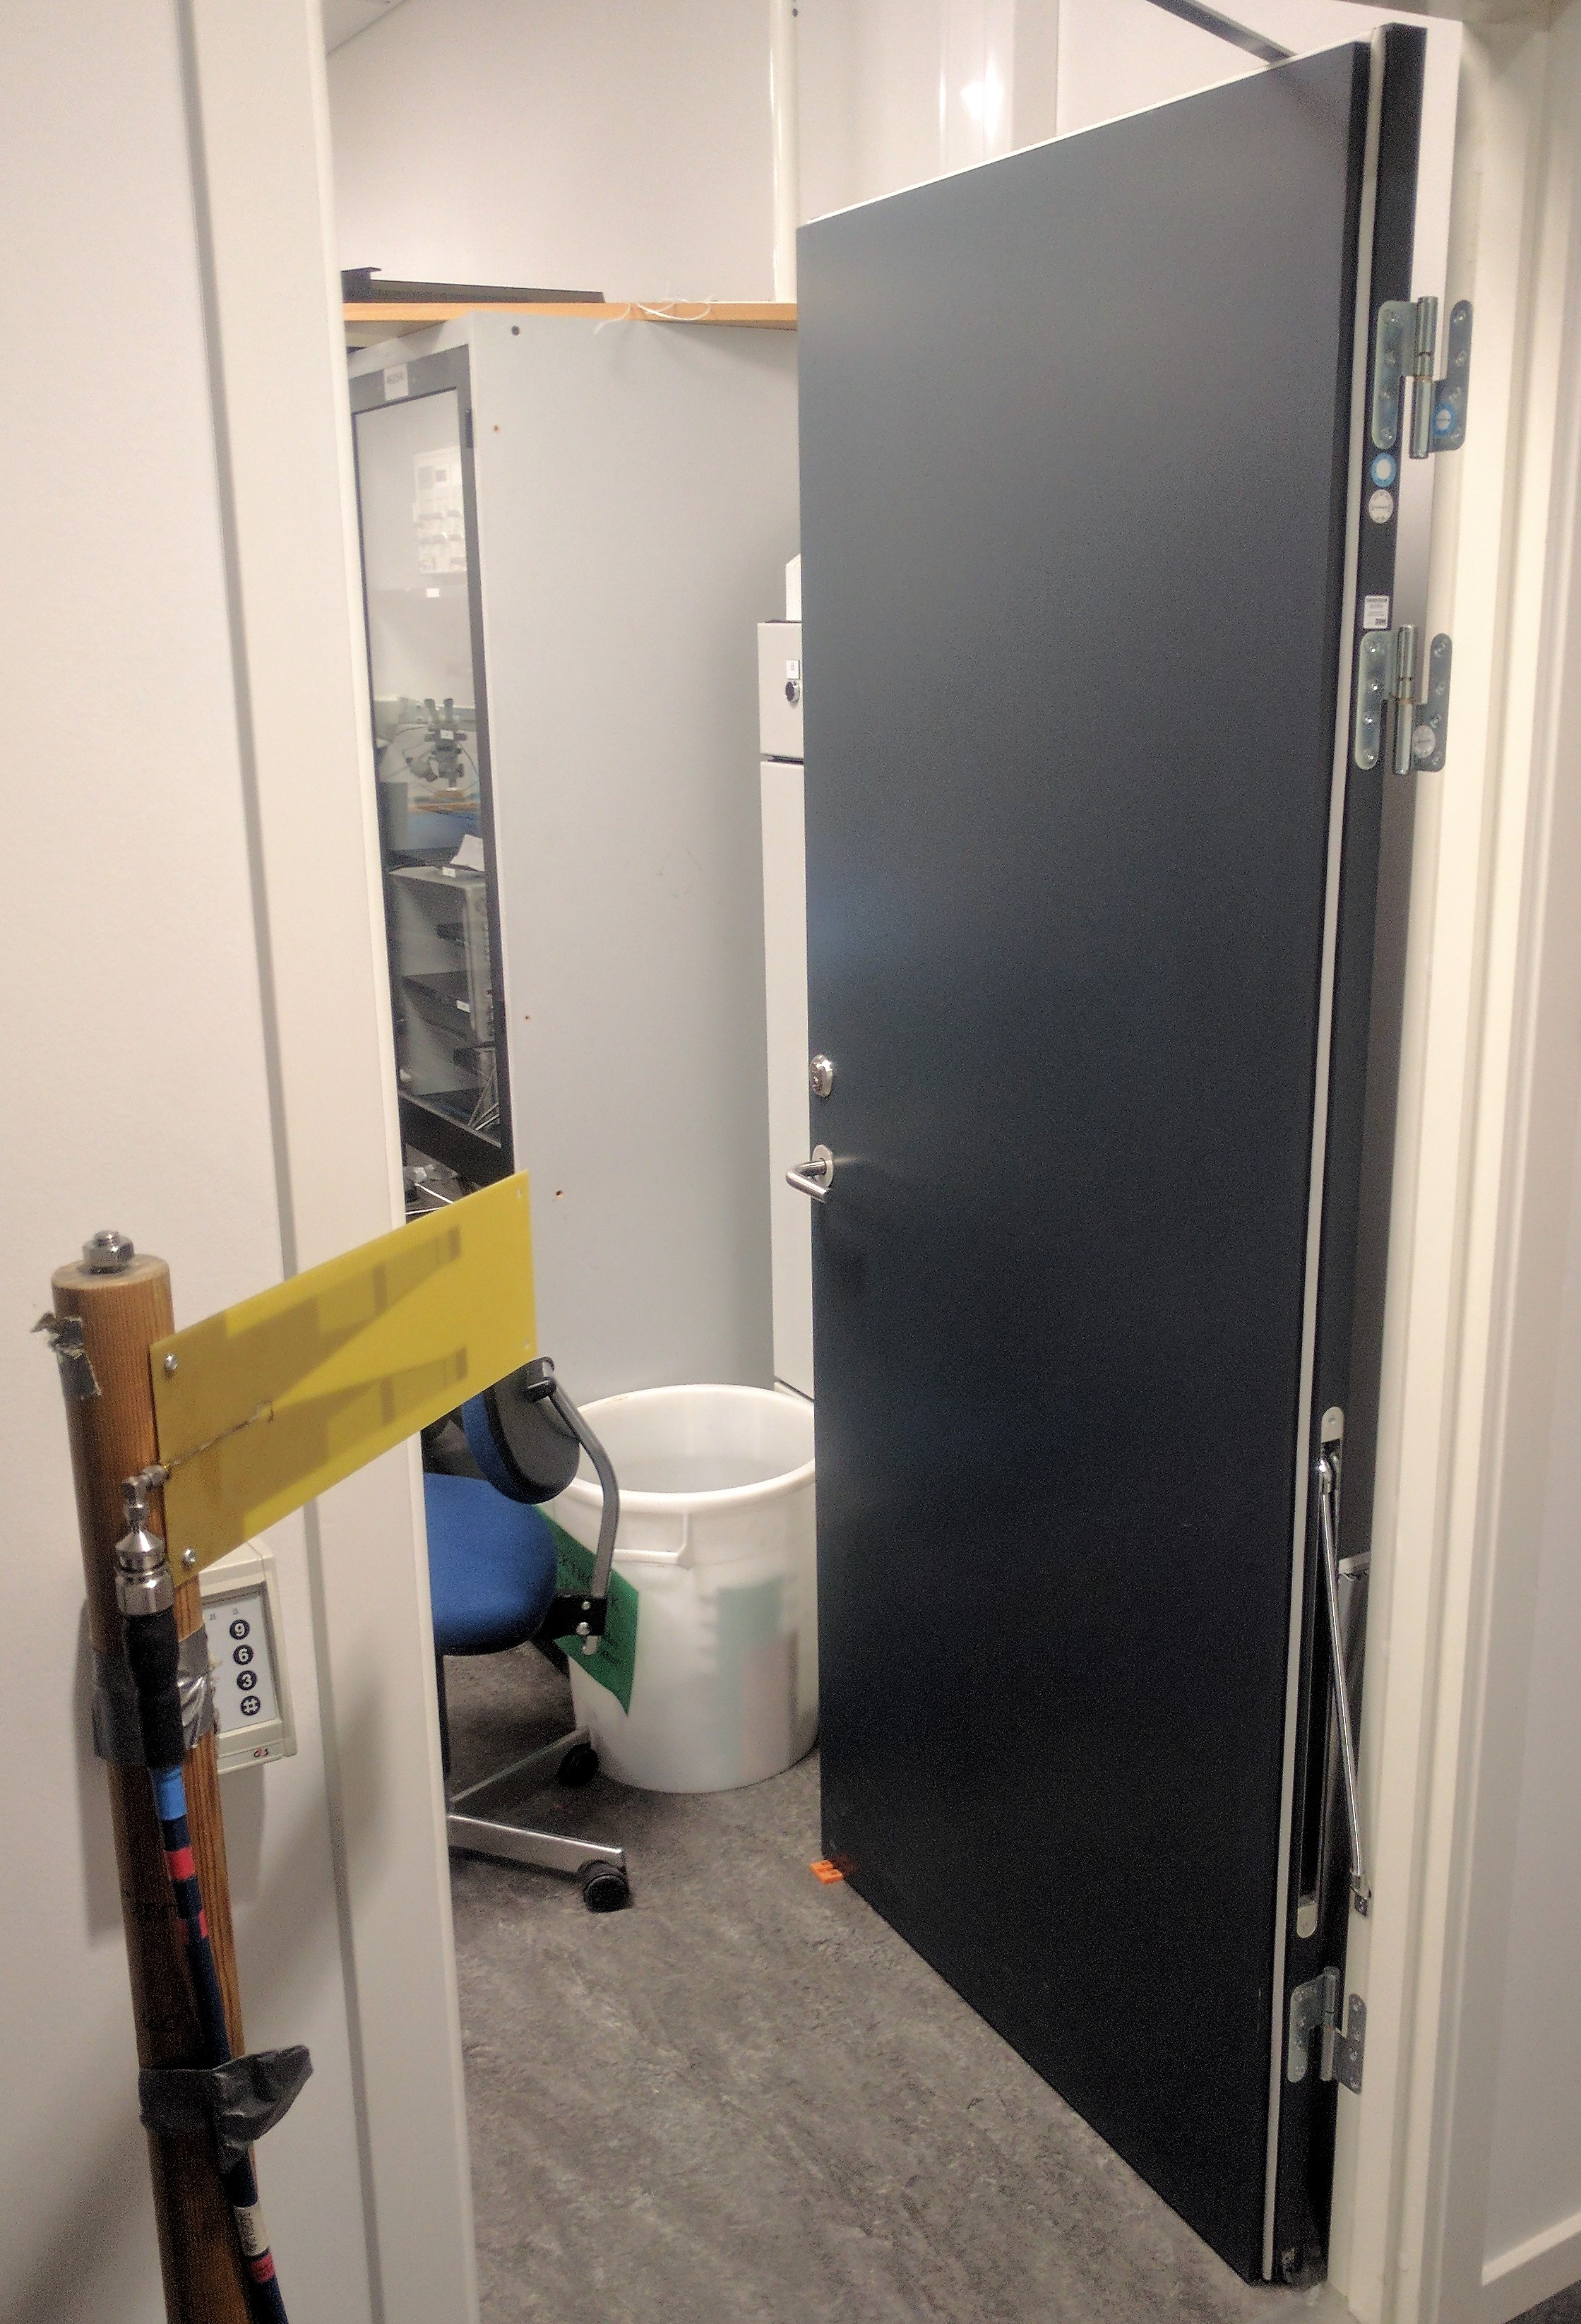
\includegraphics[width=\textwidth]{pictures/Measurement/antenna_door.jpg}
    \caption{TX antenna placement, pointing towards the door.}
    \label{antennadoor}
  \end{minipage}
  \hfill
  \begin{minipage}[H]{0.4\textwidth}
    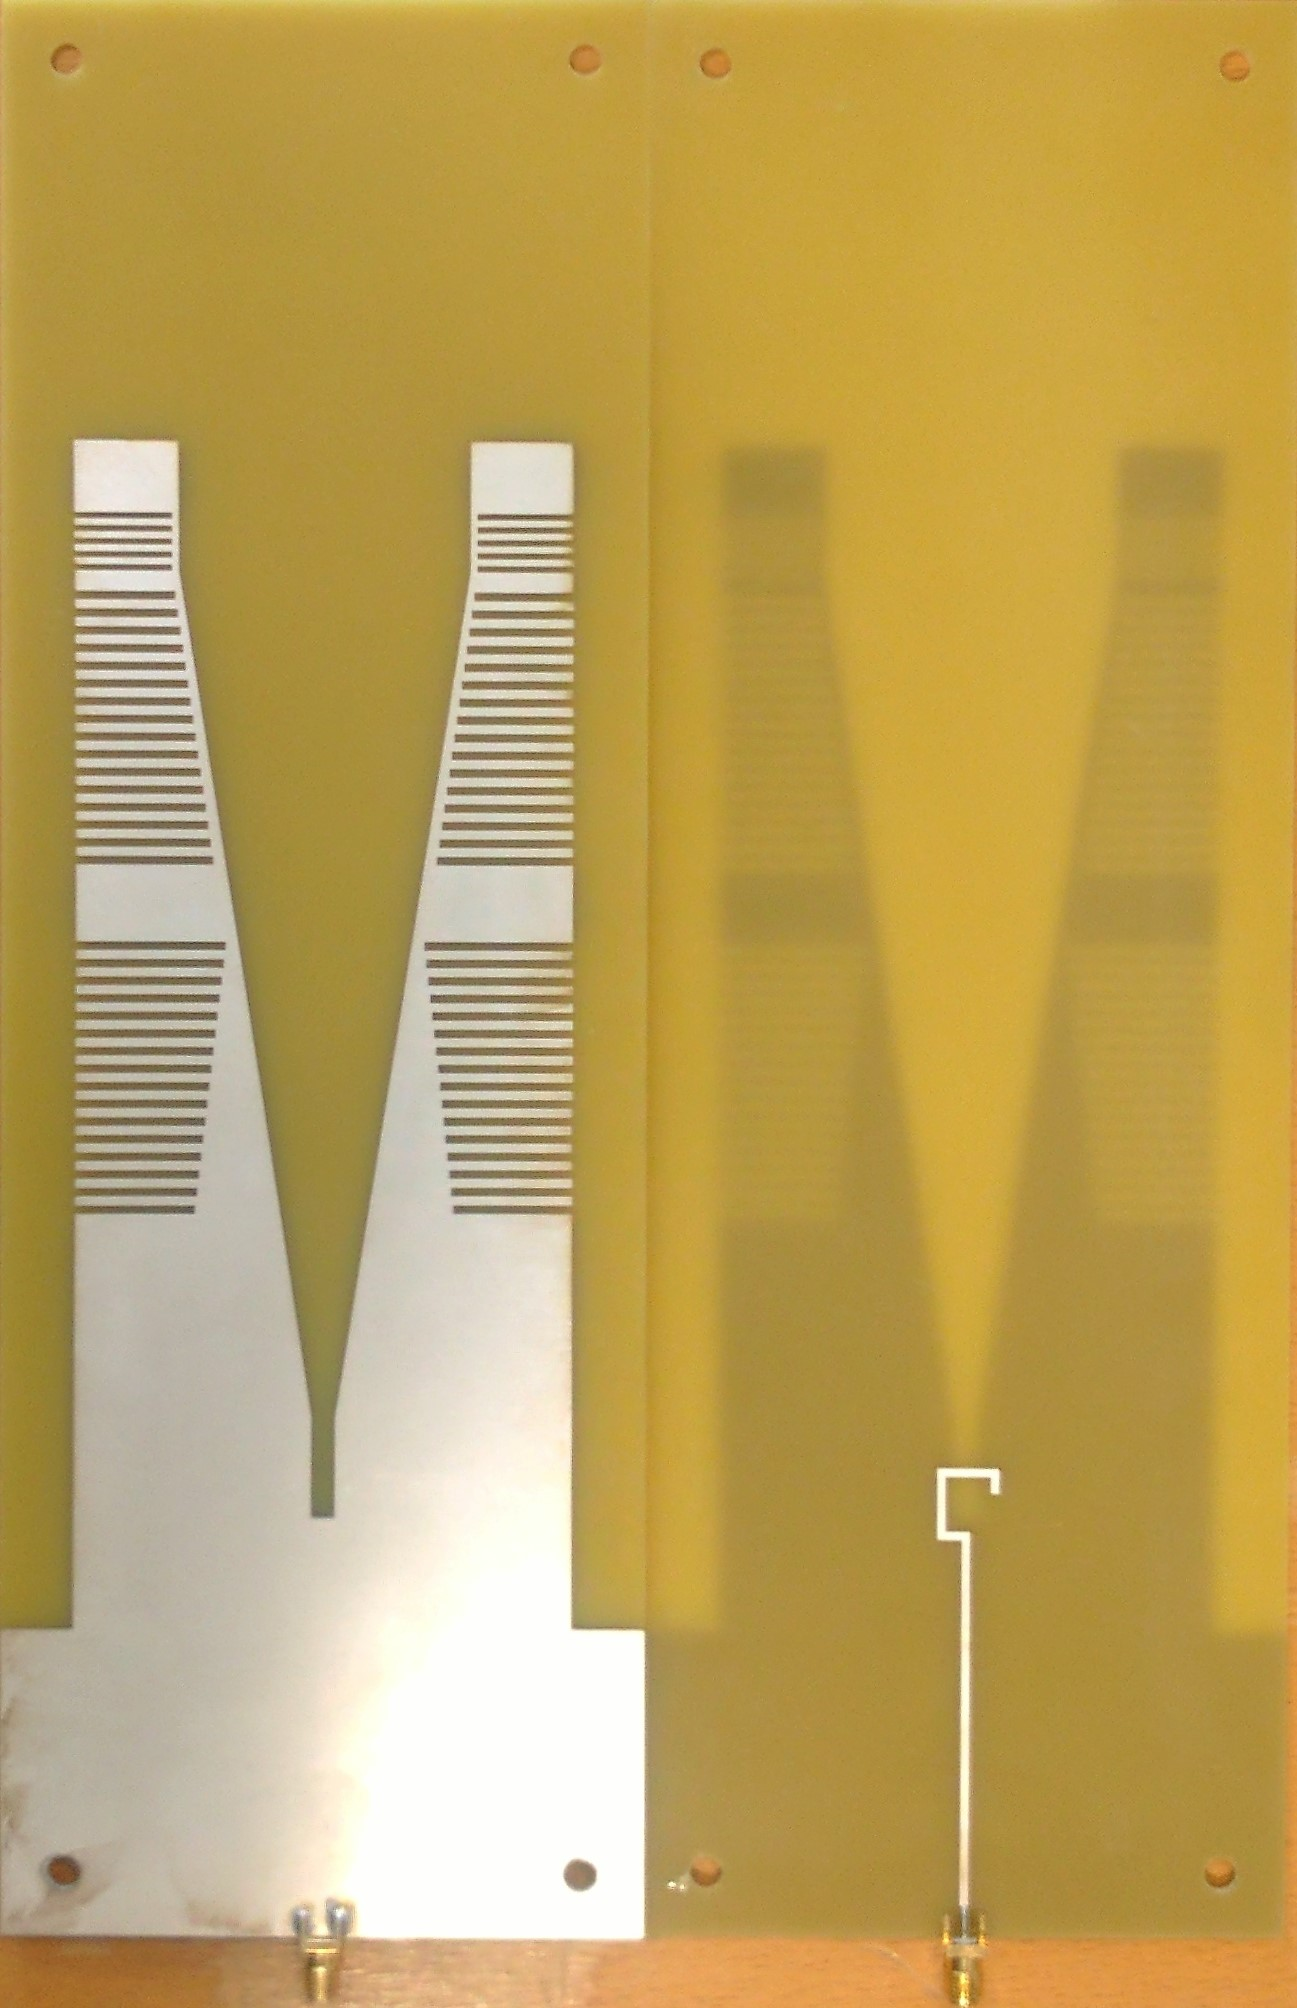
\includegraphics[width=\textwidth]{pictures/Measurement/dirrecional_antenna.jpg}
    \caption{Both sides of the directional TX antenna.}
    \label{DirAnt}
  \end{minipage}
\end{figure}

\begin{figure}[H]
\centering
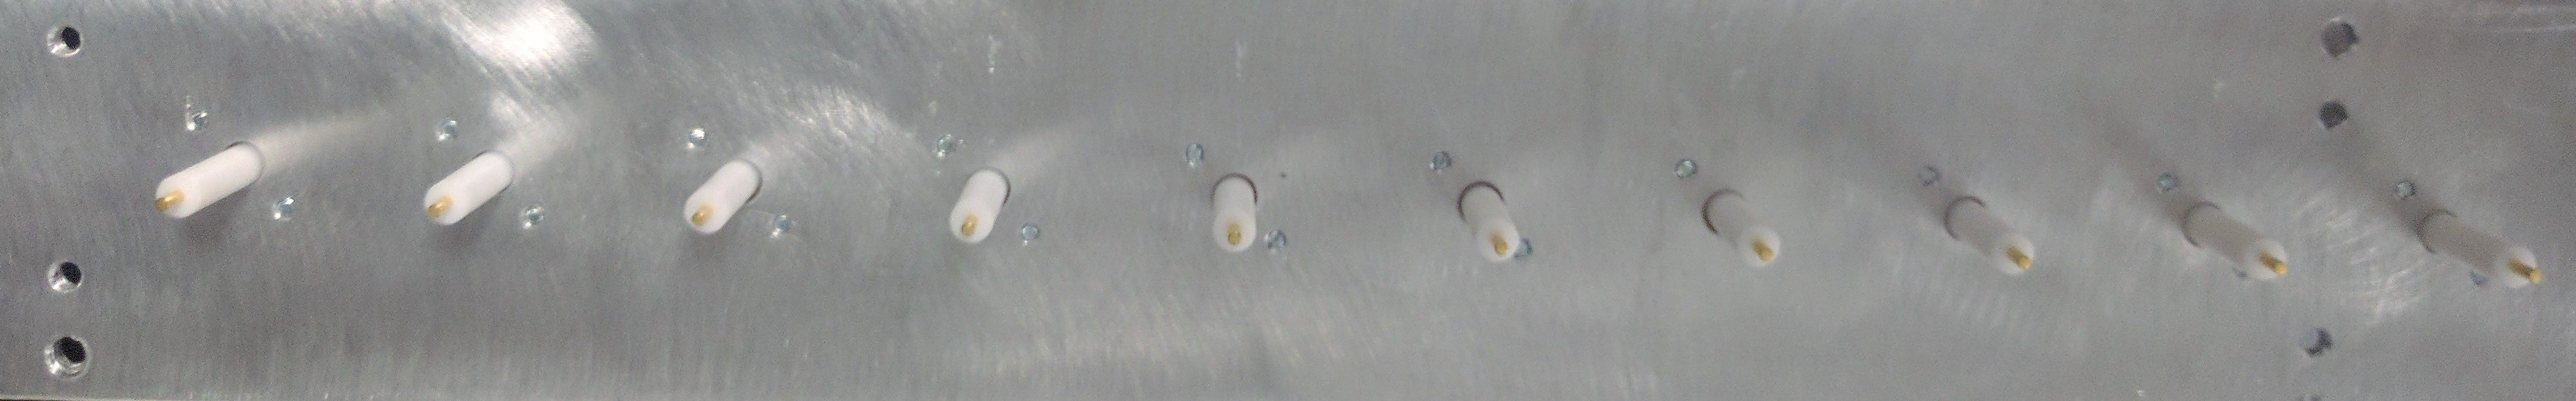
\includegraphics[width=0.7\textwidth]{pictures/Measurement/antenna_array.jpg}
    \caption{Omnidirectional RX antenna array with 2.4 cm spacing}
    \label{OmniDirAnt}
\end{figure}



\begin{figure}[H]
\centering
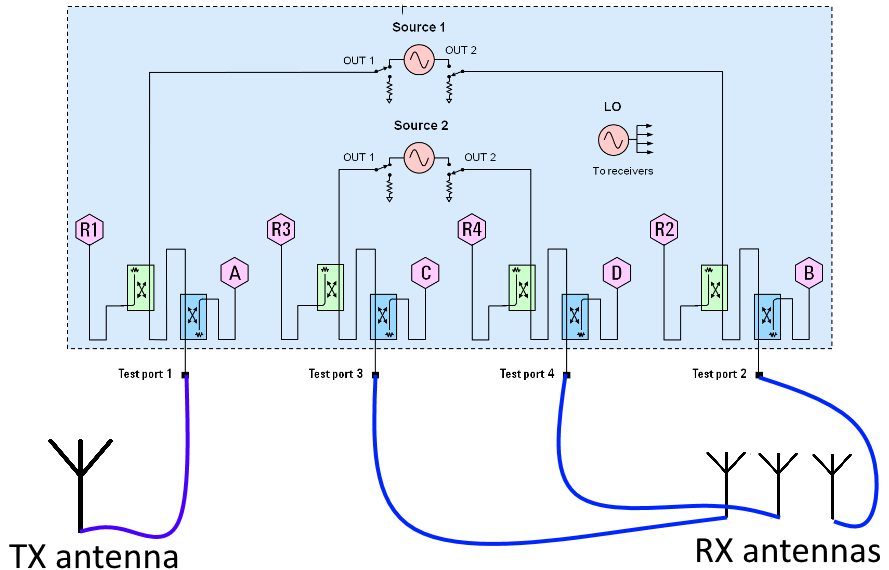
\includegraphics[width=0.65\textwidth]{figures/Gimp_figures/4portVNA.png}
\caption{The RX antennas was connected directly to the NA before the coupling (blue boxes) to reduce the attenuation. \citep{Key_PNA}}
\label{connection_diagram}
\end{figure}


%After setting up everything it was found that $P_{RX}$ was lower than expected. To increase the $P_{RX}$ the TX antenna was moved closer to the door and a shorter cable was used, this can be seen \autoref{antennadoor}. The NLOS condition was still fulfilled. 

%Keysight PNA N5527A 4-port VNA with parallel measurements and supports a frequencies from 10MHz to 67 GHz. The sweep data will me saved to a USB.
%
%Cables used have a loss of $0.5dB per m$ 
%Splitter to separate the signal to two TX antennas and point towards the doors for more equal distribution of signal.
%N5527A has a $-119dB$ noise floor without averaging with a 10Hz $IF_{bw}$ at 1-10GHz. The dynamic range of the VNA becomes:
%
%\begin{equation}
%DR = P_{tx}-119dBm 
%\label{NFvna}
%\end{equation}


%The most important part of the setup is the equipment and how they are connected. The R\&S Spectrum Analyser (model FPL9KHz-6GHz) is the center of the setup. This is the receiver of our system and gives us a readout of the spectrum in terms of power (dBm) and frequency (Hz). The two main setting on the Spectrum analyser is IF filter bandwidth and resolution. These two values gives us a sweep time.


